\documentclass[conference]{IEEEtran}
\usepackage{babel}
\usepackage[utf8]{vietnam}
\usepackage{mathtools}
\usepackage{graphicx}
\usepackage{graphics}
\usepackage{epstopdf}
\DeclarePairedDelimiter\abs{\lvert}{\rvert}
\DeclarePairedDelimiter\abst{\lvert}{\rvert^2}
\DeclarePairedDelimiter\norm{\lVert}{\rVert}
\DeclarePairedDelimiter\normt{\lVert}{\rVert^2}
\usepackage{amsfonts}

\begin{document}
	\title{Phương pháp tiền mã hóa tuyến tính MRC trong downlink thông tin di động}
	\author{Phạm Văn Nguyện\\
		MSSV: 20152737\\
		Lớp: Điện tử 02 - K60\\
		Email: nguyen.pv152737@sis.hust.edu.vn}
	\maketitle
	\begin{abstract}
		Bài viết này phân tích hiệu quả của phương pháp tiền mã hóa tuyến tính trong downlink thông tin di động với giả thiết kênh truyền là Rayleigh fading và thông tin trạng thái kênh truyền đã biết. Kết quả mô phỏng hoàn toàn phù hợp với kết quả phân tích.
	\end{abstract}
	\section{Giới thiệu chung}
	Trong hệ thống downlink thông tin di động, tín hiệu nhận được tại người dùng không những phải chịu nhiễu trên đường truyền mà còn phải chịu nhiễu giao thoa của các người dùng. Để giải quyết vấn đề này, nhiều công nghệ đã được đưa ra, một trong số đó là phương pháp tiền mã hóa. Phương pháp tiền mã hóa chia làm hai loại là tuyến tính và phi tuyến. Trong \cite{art3}, tác giả so sánh hương pháp tiền mã hóa phi tuyến dirty paper coding (DPC) với các phương pháp tiền mã hóa tuyến tính, kết quả cho thấy DPC có độ hiệu quả cao hơn nhưng độ phức tạp lớn. Một số phương pháp tiền mã hóa tuyến tính đơn giản với hiệu quả khá tốt như maximal ratio combining (MRC), zero-forcing (ZF), minimum mean-square error (MMSE) \cite{art2}. MRC ban đầu là phương pháp kết hợp anten tại bên nhận \cite{art5} với mục đích là tối đa công suất tín hiệu nhận được tại người dùng, sau đó để đơn giản về mặt công nghệ cho bên nhận người ta đưa ra phương pháp MRC precoding với cùng mục đích và được biết đến với cái tên khác là maximum ratio transmission (MRT)  \cite{art1}, đôi khi người ta dùng MRC để chỉ cả hai công nghệ này. Hiệu quả trải phổ và tốc độ dữ liệu của MRC precoding được phân tích trong \cite{art2}. Trong bài viết này, chúng ta sẽ khảo sát tỉ lệ lỗi bit BER khi hệ thống áp dụng MRC precoding. 
	\section{Mô hình hệ thống}
	Xét hệ thống downlink gồm base station với N anten phát và K user (mỗi user có  1 anten) như Hình \ref{Downlink}. 
	\begin{figure}[h]
		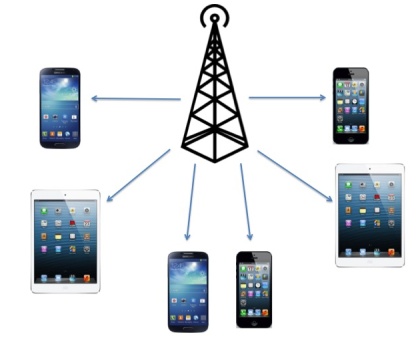
\includegraphics[width=\linewidth]{Figures/DL.png}
		\caption{Hệ thống downlink thông tin di động \cite{art2}}
		\label{Downlink}
	\end{figure}	
	\\Giả thiết rằng trạng thái kênh truyền đã biết, kênh truyền sử dụng là Rayleigh fading, ma trận kênh truyền là:
	\[H = 
	\begin{bmatrix}
	h_{11} & \dots & h_{1N}\\
	\vdots & \ddots & \vdots\\
	h_{K1} & \dots & h_{KN}
	\end{bmatrix}
	= 
	\begin{bmatrix}
	h_1\\
	\vdots\\
	h_K
	\end{bmatrix}
	\]	
	$h_i$ là vector kênh truyền có đích là người dùng thứ $i$.
	\\Tín hiệu truyền đi tại bên phát:
	\[
	s = 
	\begin{bmatrix}
	s_1 \dots s_N
	\end{bmatrix}^T
	\]
	Gọi $n$ là nhiễu Gauss trên kênh truyền, có kỳ vọng bằng $0$ và phương sai bằng $\sigma^2$:
	\[
	n = 
	\begin{bmatrix}
	n_1 \dots n_K
	\end{bmatrix}^T
	\]
	Tín hiệu nhận được tại người dùng là:
	\begin{equation}
	\label{eq1}
	y = Hs +n
	\end{equation}
	Trong phương pháp tiền mã hóa tuyến tính, người ta nhân dữ liệu cần truyền $x$ với ma trận trọng số $W$: 	
	\begin{equation*}	
	s = Wx
	\end{equation*} 
	Với:
	\[
	W = 
	\begin{bmatrix}
	w_{11} & \dots & w_{1K}\\
	\vdots & \ddots & \vdots\\
	w_{N1} & \dots & w_{NK}
	\end{bmatrix}
	=
	\begin{bmatrix}
	w_1 \dots w_N
	\end{bmatrix} 
	\]
	và:
	\[
	x = \begin{bmatrix}
	x_1 \dots x_K
	\end{bmatrix}^T
	\]
	$w_{i}$ là vector trọng số của dữ liệu gửi cho người dùng i, $x_i$ là dữ liệu cần gửi cho người dùng i.		
	Thay vào \eqref{eq1}:
	\begin{equation}
	y = HWx + n
	\end{equation}
	Mô hình hệ thống được thể hiện trong Hình \ref{SystemModel}.
	\begin{figure}[h]
		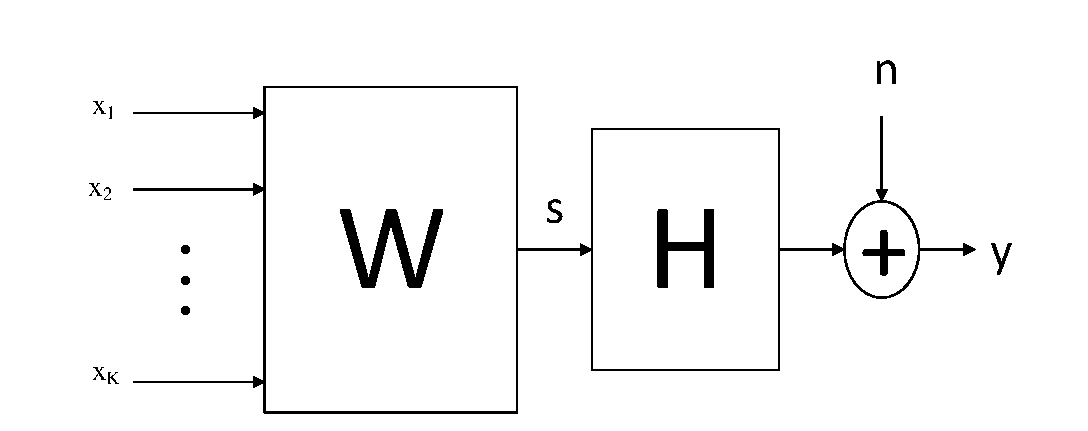
\includegraphics[width=\linewidth]{Figures/SystemModel.pdf}
		\caption{Mô hình hệ thống}
		\label{SystemModel}
	\end{figure}
	\section{MRC precoding}
	Tín hiệu nhận được tại user i là:
	\begin{equation*}
	y_i = h_iw_ix_i + \sum_{j = 1, j \ne i}^{K}{h_iw_jx_j} + n_i
	\end{equation*}
	Trong đó, $h_iw_ix_i$ là tín hiệu mong muốn, $\sum_{j = 1, j \ne i}^{K}{h_iw_jx_j}$ là nhiễu do tín hiệu của các người dùng khác, $n_i$ là nhiễu Gauss trên kênh truyền.\\
	Phương pháp MRC tối đa tỉ số SNR, tỉ số này là:
	\begin{equation*}
	\gamma = \frac{\abst{h_iw_ix_i}}{\abst{n_i}}
	\end{equation*}
	 
	Giả sử rằng $\abst{x_i} = 1$:
	\begin{equation*}
	\gamma = \frac{\abst{h_iw_i}}{\sigma^2}
	\end{equation*}
	Ta cần xác định $w_i$ sao cho $\gamma$ lớn nhất với giả thiết đã biết $h_i$.
	Áp dụng bất đẳng thức Cauchy - Schwarz:
	\begin{equation*}
	\abst{h_iw_i} \le \abst{h_i} \abst{w_i} 
	\end{equation*}
	Dấu $"="$ xảy ra khi $w_i = \alpha h_i^H$.\\
	$h_i^H$ là vector liên hợp phức chuyển vị của $h_i$.\\
	$\alpha$ là hệ số tỉ lệ.
	\section{Kết quả mô phỏng}
	Trong phần này, chúng ta sẽ xét hệ thống chỉ có một user, phương pháp điều chế là BPSK. Kết quả mô phỏng được thể hiện trong Hình \ref{EbN0} và Hình \ref{Tx}.\\
	\begin{figure}[h]
		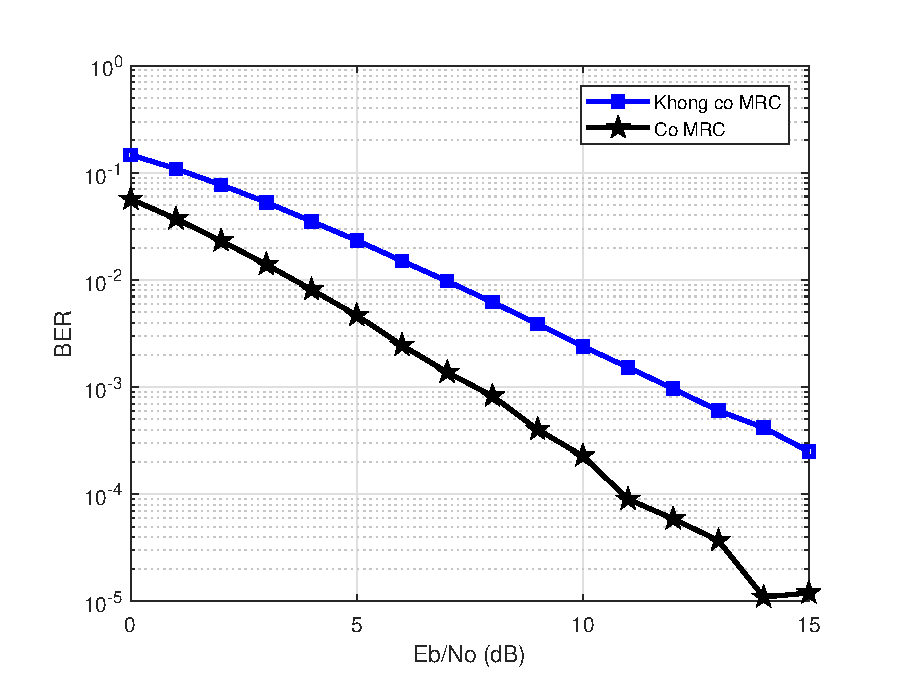
\includegraphics[width=\linewidth]{Figures/EbN0}
		\caption{Tỉ lệ lỗi bit BER khi thay đổi Eb/N0 (3 anten phát) }
		\label{EbN0}
	\end{figure} 
	\begin{figure}[h]
		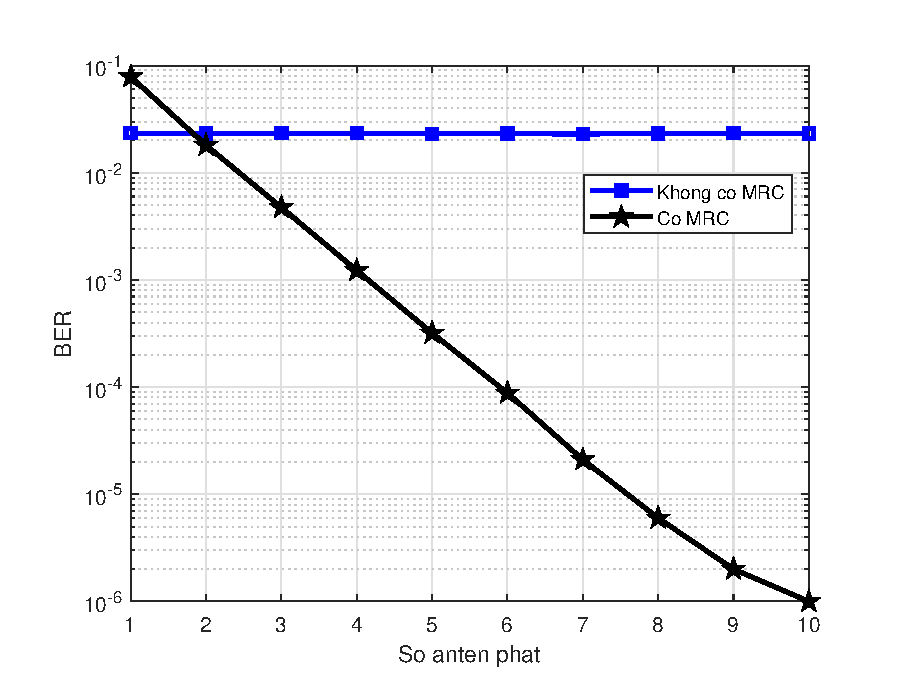
\includegraphics[width=\linewidth]{Figures/Tx}
		\caption{Tỉ lệ lỗi bit BER khi thay đổi số anten phát (Eb/N0 = 5 dB) }
		\label{Tx}
	\end{figure}
	Từ kết quả mô phỏng, ta có thể thấy rằng tỉ lệ lỗi bit BER giảm khi tăng tỉ số Eb/N0 và số anten phát.
	\section{Kết luận}
	Như vậy, chúng ta đã phân tích hiệu quả của phương pháp MRC precoding. Tuy nhiên, nhược điểm của phương pháp này là không xem xét đến nhiễu giữa các người dùng, do đó khi có nhiều người dùng, ta cần có phương pháp khác.
	\section{Tài liệu tham khảo}
	\bibliographystyle{IEEEtran}
	\bibliography{tailieuthamkhao} 
\end{document}